\documentclass{beamer}
\usetheme[colour=UoEblue]{UsherNew}
%% Alternative options are:
%\usetheme[colour=USHERgreen]{UsherNew}
%\usetheme[colour=USHERblue]{UsherNew}
\usepackage{beamernotes}
\usepackage{amsmath}
\usepackage{pgf,tikz,pgfplots}
\pgfplotsset{compat=1.15}
\usepackage{mathrsfs}
\usetikzlibrary{arrows}
\pdfcompresslevel=9
\pdfobjcompresslevel=3

\title[]{Decrypting Elliptic Curves...}
\subtitle{Decrypting Elliptic Curves...}
\author{Benjamin Brown}
%\institute{Institute Name}
\date{3\textsuperscript{rd} July 2020}

\begin{document}

\definecolor{fuqqzz}{rgb}{0.9568627450980393,0,0.6}
\definecolor{ccqqqq}{rgb}{0.8,0,0}
\definecolor{ffzzqq}{rgb}{1,0.6,0}
\definecolor{xdxdff}{rgb}{0.49019607843137253,0.49019607843137253,1}

\begin{frame}
  \titlepage
\end{frame}
\bnote{This generates notes for pdfpc. These notes also appear
  on the handout/article versions.}

\begin{frame}[t]{Ellipses}
	After circles, ellipses are the most familiar curves in mathematics.
	\begin{figure}[h]
		\centering
		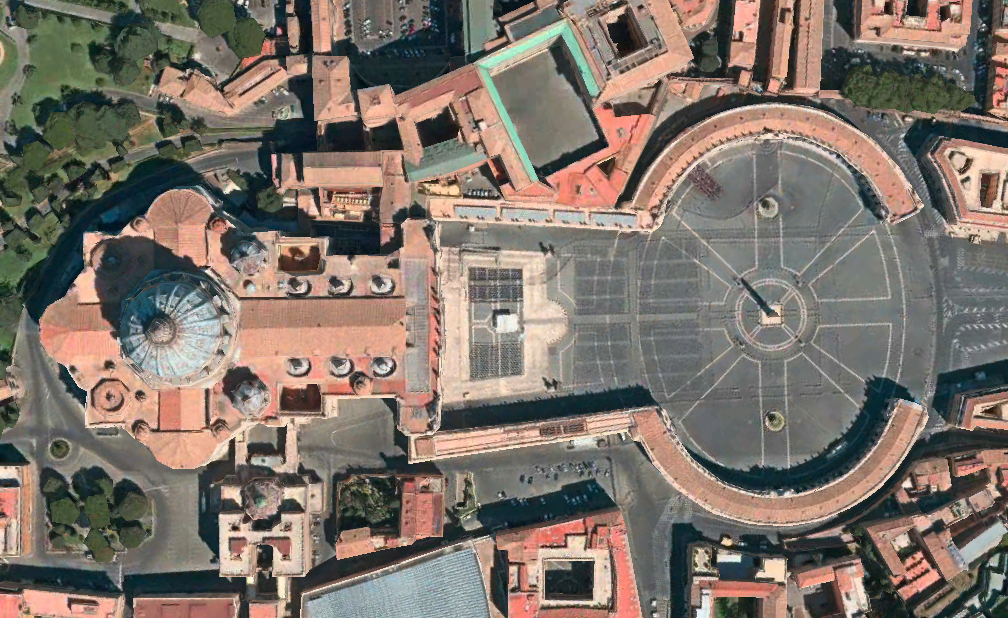
\includegraphics[width=10cm]{st-patricks-square}
		\caption{St Patrick's Square.}
	\end{figure}
\end{frame}

\begin{frame}	
	copy page over
\end{frame}

\begin{frame}[t]{Elliptic Functions}
	Arc-length of an ellipse?
\begin{equation*}
	x = a\cos\theta,\quad y=b\sin\theta\quad \quad \quad 
\end{equation*}
	
\begin{equation*}
	\begin{split}
		L &= \int_{0}^{2\pi} \sqrt{ ( \partial_{\theta}x )^{2} + ( \partial_{\theta}y )^{2} }\, d\theta \\
		&= 4a \int_{0}^{1} \sqrt{ 1 - k^{2} u^{2} }\, du \quad (k^{2} = (a^{2} - b^{2})/a^{2};\quad u = \sin\theta ) \\
		&= \frac{1}{2} \int_{1-k^{2}}^{1} \frac{t\, dt}{\sqrt{t(t-1)(t - (1-k^{2}))}}\quad (t = 1 - k^{2}u^{2})
	\end{split}
\end{equation*}	
\end{frame}

\begin{frame}
	Integrals of the form
	\begin{equation*}
		w = f(z) = \int_{P}^{z} \frac{t\, dt}{c_{3}t^{3} + c_{2}t^{2} + c_{1}t + c_{0}}
	\end{equation*}
	are called \emph{elliptic integrals (of the 2\textsuperscript{nd} kind)}. \\~\\
	
	In general, involve integrals with square-roots of cubic or quartic polynomials. \\~\\
	
	\emph{Elliptic functions} are the inverses to elliptic integrals, $z = f^{-1}(w)$. \\~\\
		
	They have no solution involving only elementary functions.
\end{frame}

\begin{frame}
	Denominator is the \emph{square-root} of:
	\begin{equation*}
		E: \quad y^{2} = x(x-1)(x-\lambda).
	\end{equation*}
	Over $\mathbb{C}$, it is the equation for a \emph{Legendre form} elliptic curve. \\~\\
	
	Problem: there is no single-valued function $y = \pm\sqrt{f(x)} = \pm\sqrt{x(x-1)(x-\lambda)}$ on the whole of $\mathbb{C}$. \\~\\
	
	$$
		\pi : E \rightarrow \mathbb{C}\cup \{\infty\}; \qquad (x,y) \longmapsto x; \qquad \pi^{-1}(x) = \begin{cases}
		\big\{ y = + \sqrt{f(x)} \big\}, \\
		\big\{ y = - \sqrt{f(x)} \big\}.
		\end{cases}
	$$
\end{frame}
	
\begin{frame}
	To remedy this, note that away from $0, 1, \lambda, \infty$, square root $y = \sqrt{f(x)}$ has two single-valued determinations on $\mathbb{C} \cup \{\infty\}$. \\~\\
	
	Join them together via cuts from $0$ to $1$, and from $\lambda$ to $\infty$: \\~\\
	
	So we now have a surface (a torus) on which $\sqrt{f(x)}$ 
	
	
\end{frame}

\begin{frame}	
	(Figure)
\end{frame}

\begin{frame}
	Have a map
	$$
		E(\mathbb{C}) \longrightarrow \mathbb{C}/(\omega_{1}\cdot \mathbb{Z} + \omega_{2}\cdot \mathbb{Z} ).
	$$
	Right-hand side is an abelian group, \emph{a torus}. \\~\\
	
	Does the elliptic curve $E(\mathbb{C})$ have an abelian group structure?
\end{frame}

\begin{frame}[t]{The Group Law}
	Property of a cubic curve $E$: any line $L$ intersects $E$ in at most 3 points. \\~\\ 	
	
	Pick a marked point $\mathcal{O} \in E$ to serve as the identity (usually $\infty$ is chosen).
\end{frame}

\begin{frame}[t]{Point at Infinity}
	``\emph{Homogenise}'' the equation:
	$$
		y^{2} = x(x-1)(x-\lambda) \longmapsto y^{2}z = x(x-z)(x-\lambda z).
	$$
	I.e., introduce powers of a new coordinate $z$ so every term has degree 3. \\~\\
	
	Point at infinity gotten from setting $z = 0$: $\infty \in \big\{ y^{2}\cdot 0 = x(x-0)(x-\lambda\cdot 0) \big\} \implies x = 0$.
\end{frame}

\begin{frame}{Finite Fields}
	Point addition can be defined over any field. \\~\\
	
	A field is a ``nice'' ring, \emph{e.g.} $\mathbb{Q}, \mathbb{R}, \mathbb{C}$. These are \emph{infinite fields}. \\~\\
	
	There are also \emph{finite fields}, say $\mathbb{Z}_{2}, \mathbb{Z}_{3},\ldots$. \\~\\
	
	In general $\mathbb{Z}_{p^{k}}$, with $p$ a prime number and $k\geq 1$, are all fields. \\~\\

	In $\mathbb{Z}_{p}$ arithmetic is done modulo $p$. \\~\\
	
	E.g., time on a digital clock face is read modulo 24, so that $25:00 \equiv 01:00$, etc.
\end{frame}

\begin{frame}
	Elliptic curves look very different over a finite field $\mathbb{F}_{p}$!	
\end{frame}

\begin{frame}[t]{Cryptography}
	Cryptography is the process of writing using various methods, ciphers, to keep messages secret. \\~\\
	
	Example: Caesar Cipher (very insecure!) \\~\\
	\begin{itemize}
		\item Each letter in the message is shifted 3 letters along.
		\item ``Decrypting elliptic curves'' $\mapsto$ ``Ghfubswlqj hoolswlf fxuyhv''.
		\item To Decrypt, just undo the shift. \\~\\
	\end{itemize}
\end{frame}

\begin{frame}[t]{Diffie-Hellman Key Exchange}
	A method of exchanging secret information over unsecure channels. \\~\\
	
	Alice and Bob each have a secret key, $a, b \in \mathbb{Z}$, and they agree on an elliptic curve $E$ and point $\mathcal{O}$. \\~\\
	
	Alice sends to Bob the point $a \cdot \mathcal{O}$, and Bob sends to Alice the point $b \cdot \mathcal{O}$ (these are public keys). \\~\\
	
	Alice then calculates $a \cdot b \cdot \mathcal{O}$, and likewise Bob calculates $b \cdot a \cdot \mathcal{O}$, which are equal as $E$ is an abelian groups. \\~\\
	
	So they now have a shared secret key $a \cdot b$
\end{frame}

\begin{frame}[t]{Discrete Logarithm Problem}
	Someone observing this exchange would only know what $E$, $\mathcal{O}$, $a\cdot \mathcal{O}$, and $b\cdot \mathcal{O}$ are. \\~\\
	
	
	
\end{frame}

\begin{frame}
\end{frame}

\begin{frame}
\end{frame}

\begin{frame}
\end{frame}

\begin{frame}
\end{frame}

\begin{frame}
\end{frame}

\begin{frame}
\end{frame}

\begin{frame}[t]{Another Form}
	Legendre form only one of infinitely many forms for an EC. \\~\\

	Another fun one is the \emph{Hesse cubic}: 
	$$
		f(x,y,z) = x^{3} + y^{3} + z^{3} - 3\lambda xyz = 0.
	$$
	Hessian curve 
	$$
		\det ( \partial^{2} f / \partial x_{i}x_{j} ) \propto f(x,y,z),
	$$
	and they intersect each other 9 times in general. 
\end{frame}



\end{document}
